% Los objetivos específicos de cada uno de los subproyectos participantes, enumerándolos brevemente, con claridad, precisión y de manera realista (acorde con la duración prevista del proyecto).
%
% En los subproyectos con dos investigadores principales, deberá indicarse expresamente de qué objetivos específicos se hará responsable cada uno de ellos.

\subsubsection*{Objectives of the \BATA\ subproject}

\begin{figure}
\begin{center}
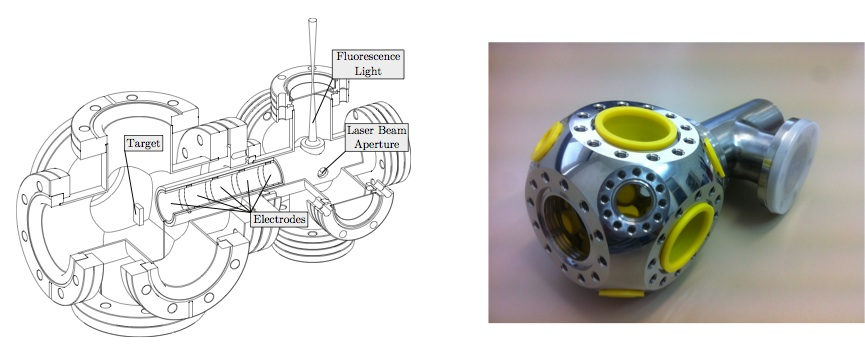
\includegraphics[width=0.99\textwidth]{img/BChamber.jpg}
%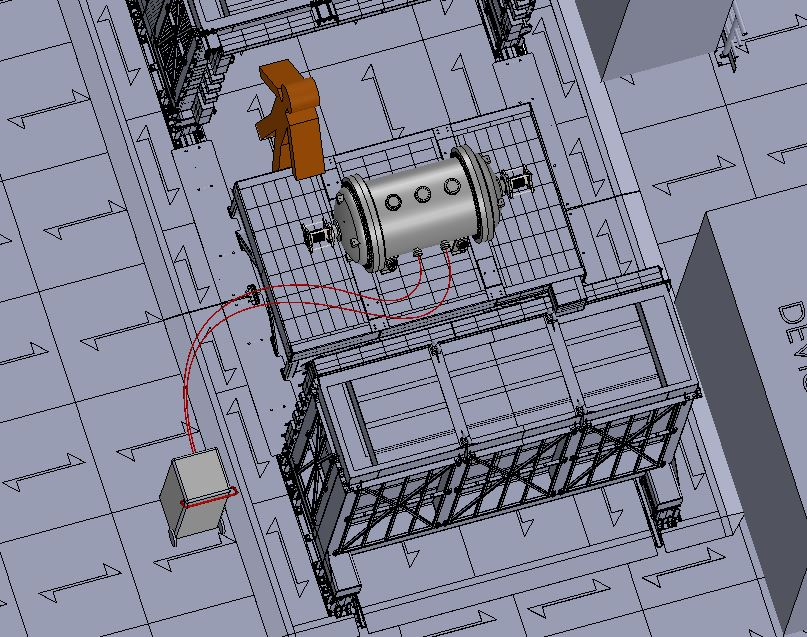
\includegraphics{img/CALIB_LSC_sources.jpg}
\caption{\small Left. A diagram of the chamber for the \BATA\ prove-of-concept experiments: right: the camber, built at IFIC, and ready to be installed at CLPU.}
\label{fig:chamber}
\end{center}
\end{figure}

The \BATA\ subproject will focus in the R\&D program needed to clearly establish the feasibility of tagging (e.g., detecting) the barium (Ba$^{++}$) ion produced in the double beta decay of xenon. 
%Demonstrating that an efficient detection of barium is possible in an \HPXE\ would imply that the NEXT technology could be upgraded to the ton scale while at the same time reducing the background by two or more orders of magnitude, resulting in a virtually background-free experiment with enormous possibilities of hitting a discovery. 

The \BATA\ program involves a set of proof-of-concept experiments. It also proposes the developments of a 4.1 $\mu$m laser, needed for the deshelving of the metastable state. An attractive feature of such laser is its wide range of scientific and technological applications. CLPU is specially well suited to develop the technology.

The different objectives of this subproject are, therefore:

\begin{itemize}
	\item \textbf{Proof of principle experiment with Ba ions generated by means of an electrical discharge.}
In a first round of experiments we will excite resonantly the S$\leftrightarrow$P transition of Ba$^+$ ions generated by an electrical discharge between two barium electrodes and will collect the fluorescence signal of the P$\rightarrow$D transition. Although this generation method is not ideal because several different species different from Ba ions will be generated (e.g., molecules like BaO or clusters), it does not need a major technological development. 

The laser source needed to resonantly excite the $Ba^{+}$ must have a wavelength of 493.5\,nm, not available in commercial lasers. {em The laser source will, therefore be produced at the CLPU}, optimising a tuneable Ti:sapphire laser at 987\,nm to obtain second harmonic generation (SHG) at 493.5\,nm. This setup allows the tuning of the wavelength and control the bandwidth of the laser which is necessary to precisely tune it to the transition frequency (e.g. to correct for pressure broadening and other effects). The IFIC group, on the other hand, has fabricated the test chamber needed for the experiments 
(see Figure \ref{fig:chamber}). 

It is expected that these initial set of experiments will provide valuable information about the population dynamics in Ba$^+$ ions, and the influence of the different homogenous and in-homogenous broadening mechanisms. 
	
	\item \textbf{Proof of principle experiment with Ba ions generated by an ion source.}	
In this objective, in order to get a better approximation of the final conditions of NEXT experiment a source of ions will be designed and constructed at the CLPU. This ion source will be based on selective ionisation and mass spectrometry techniques, and it will allow an efficient selection of the desired target species (e.g, $Ba^{+}$~and $Ba^{++}$). With this setup we will be able to study the recombination process Ba$^{++}\rightarrow$Ba$^{+}$ and decide whether it can be induced by collisions with xenon atoms or requires an additive (see discussion in the objectives of the CALREC subproject). Depending on the results of the experiment, a magnetic trap can bee added to improve the experimental conditions. 
	
%	\item \textbf{Proof of principle experiment with Ba ions generated by an ion source and with a magneto trap.}	
% In order to better control the experimental conditions, we will repeat the experiment but with the ions now confined in a magnetic trap. This trap will allow us to have an excellent degree of control over the experimental conditions and to approach the conditions that can be expected in the NEXT experiment. For instance we will carry out different measurements comparing the collected fluorescence signal as a function of the pressure of the Ba$^+$ ions and the pressure of the surrounding environment. These measurements are mandatory because the population dynamics is very sensitive to pressure, i.e., to collisions. 
%	
	\item \textbf{Proof of principle experiment with an additional laser for deshelving the D state.}
A likely scenario is that the collisional induced decay between the metastable state D and the ground state S is either not effective or too slow for obtaining an appreciable fluorescence signal. In this situation the population is trapped in the metastable state D  and the fluorescence cycle can not be closed. To avoid this difficulty our approach will be to use a second laser to induce a two photon transition (one photon is forbidden by selection rules, between the states D and S, see Fig.\,\ref{fig.BATA}). 

\item \textbf{Development of a state-of-the-art 4.1\,$\mu$m laser}. The laser needed for
deshelving the D state must have a wavelength of around 4.1\,$\mu$m. While small commercial laser system exists in this range, (we will purchase one of them for the experiment described in the previous paragraph), no commercial system will satisfy the conditions of power and stability needed for a real \BATA\ experiment. Furthermore, such a laser, already well in the infrared region, has many potential applications.	

There are only a few laser systems that generate laser emission in the mid-infrared (MIR, from 2 to 10\,$\mu$m). There are lasers that emit in discrete wavelengths as gas lasers ($CO_2$, Xe-HE, He-Ne), chemical lasers (Hidrogen Fluoride, Deuterium Fluoride) and Dye lasers by Raman Shift. All this systems are big and complex, emit in relative low power and are involve the use of dangerous materials (chemicals, flammable gases and/or carcinogenic powders). 

A much more interesting alternative to reach the desired MIR wavelength is the use of an optically pumped solid state laser (OPSSL) system, by means of a specific doping of crystals with metal transition ions. Wavelengths of 2 and 2.9\,$\mu$m are available with $Tm^{3+}$, $Tm^{3+}$-$Ho^{3+}$ and $Er^{3+}$ active ions in crystalline matrices. Recent developments involve doping with $Cr^{2+}$ and $Fe^{2+}$ ions. This should allow to develop a laser system that emits in a broad range: 2.1 to 3\,$\mu$m and 3.7 to 5\,$\mu$m, respectively. Another option is to work with quantum cascade semiconductor systems potentially available from 3.8 to 9.5\,$\mu$m in a discrete range, i. e.  not only continuously. 

To develop a laser system around 4.1\,$\mu$m we need to study and evaluate the best optical parameters of some materials (crystalline matrices or semiconductors) that can be used as active laser materials.  This will allow us to design a laser cavity with the appropriate  optical components and devices (these should work in the MIR region). It will also allow us to maximise the efficiency of the laser system. The cavities are different for systems optically pumped (the case of crystals doped with $Cr^{2+}$ o $Fe^{2+}$) or electrically pumped (as the quantum cascade semiconductors). These cavities can be 2-, 3- or 4- folded mirror configurations depending on the advantages observed during the design using optical and numerical software. The characterisation of the laser emission and other related parameters will allow us  to improve the laser system to use in the NEXT experiment. 

\end{itemize}

%\subsubsection*{\BATA\ subproject: Resources}
%
%For the successful development of this subproject, CLPU will provide the required human and technological resources. CLPU is the centre of reference in Spain regarding laser technology, and takes active part in several international and national projects. The leader of this subproject will be Alicia V. Carpentier who has a well recognised international trajectory in laser-matter interaction. Moreover, {\bf CLPU considers this project of high priority and consequently will offer the collaboration of all the scientific department} consisting of a multidisciplinar team with broad experience in laser technology and development, and laser-matter interaction. 
%
%Furthermore, CLPU will support this project with some of the already operating laser systems in its installation. This is extremely important because such systems usually cost of the order of several hundreds of thousand euros. The human resources needed to operate the laser systems will be provided by CLPU as well. For the construction of the ion source, and taking into consideration the specific requirements of this development, we will apply for an \emph{EXPLORA tecnología} in the 2014 call. 
%
%The budget of this subproject will be dedicated to: a) purchase small equipment for the proof-of-principle experiments; b) purchase a small commercial infrared laser for the initial deshelving experiment; c) develop a state-of-the-art, high power, very stable infrared laser to be used in a large system. It is important to insist that such a laser has many possible applications given the fact that its wavelength is not absorbed by the atmosphere as it lies in what is called the infrared atmospheric window.
%
%
%\subsubsection*{BATA subproject: schedule}
%
%
%
